% Fakesection 序言之前

\RequirePackage[l2tabu, orthodox]{nag}
\RequirePackage{ifxetex}
\RequireXeTeX

\documentclass{ctexart}

%颜色
\usepackage{xcolor}

%长度
\usepackage{printlen}
\uselengthunit{mm}

%图形
\usepackage{pifont}
\usepackage{ean13isbn}
\usepackage{qrcode}
\usepackage{pdfpages}
\usepackage{overpic}
\usepackage{graphicx}
\graphicspath{{./src/}}
\usepackage{media9}
\usepackage{wallpaper}
\usepackage{wrapfig}

%表格
\usepackage{tabu}
\usepackage{longtable}
\usepackage{booktabs}
\usepackage{diagbox}
\usepackage{multicol}
\usepackage{multirow}
\usepackage{makecell}
\usepackage{fancybox}
\usepackage{colortbl}
\usepackage{tcolorbox}
\tcbuselibrary{skins}
\tcbuselibrary{breakable}
\tcbuselibrary{theorems}
\tcbuselibrary{listings}
\tcbuselibrary{xparse}
\tcbuselibrary{minted}% 用minted排版代码
\usepackage{fvextra}
\usepackage{csvsimple}
\usepackage{boxedminipage2e}

%公式
\usepackage{amsmath}
\usepackage{amsthm}
\usepackage{amsfonts}
\usepackage{amssymb}
\usepackage{amsbsy}
\usepackage{amsopn}
\usepackage{amstext}
\usepackage{mathrsfs}
\usepackage{bm}
\usepackage{textcomp}
\usepackage{latexsym}
\usepackage{exscale}
\usepackage{relsize}
%\usepackage{xymtex}
\usepackage{physics}
\usepackage{siunitx}
\usepackage{hologo}
\usepackage{cases}

%文字
\usepackage{csquotes}
\usepackage{microtype}

%正文
\usepackage{fancyhdr}
\usepackage{geometry}
\usepackage{lastpage}
\usepackage{indentfirst}
\usepackage{setspace}
\renewcommand\arraystretch{1.5}

%非正文
\usepackage{makeidx}
\makeindex
\usepackage{epigraph}
\usepackage{varwidth}
\usepackage{exercise}
\usepackage{tasks}
\renewcommand{\ExerciseName}{问题}
\renewcommand{\AnswerName}{回答}
\renewcommand{\listexercisename}{问题}

%参考文献
\usepackage{morewrites}
\renewcommand{\thefootnote}{\fnsymbol{footnote}}
\usepackage[resetlabels]{multibib}

%标题
\usepackage{caption}
\usepackage{subcaption}
\DeclareCaptionLabelFormat{andtable}%
{#1#2~\&~\tablename\thetable}
\newcounter{sub}

%其它
\usepackage{atbegshi}
\usepackage{lipsum}

\csname
endofdump
\endcsname

%代码
\usepackage{minted}
\usepackage{boxie}
\makeatletter
\xdefinecolor{tcbcol@back}{rgb}{0,0,0}
\makeatother
\usepackage{tikz}
%%MatLab命令行
\newcommand{\MatlabLogo}{%
	\begin{tikzpicture}[x=2.4ex,y=2.4ex,line width=0ex,scale=1]
		\node[draw,fill=white,text=white] at (0, 0) (a) {
				\includegraphics[width=2.4ex]{matlabLogo.ai}
			};
	\end{tikzpicture}
}
\tcbset{%
	skin=enhanced,%
	matlab/.style={%
		skin=bicolor,%
		boxrule=0.1mm,%
		%toptitle=1ex,
		sharp corners,
		breakable,%
		colbacktitle=WinGray,%
		colframe=WinGray,%
		coltitle=black,%
		fonttitle=\sffamily,%\bfseries,
		fontupper=\small\sffamily,
		fontlower=\small\sffamily,
		frame style={%
			draw=WinBlue,%
			left color=WinBlue,%
			right color=WinBlue%
		},%
		overlay unbroken = {%
			\node[inner sep=0pt,anchor=north west,yshift=-3pt,xshift=1.2pt,text=black]
			at (frame.north west){\MatlabLogo};% \fbox{\faTerminal}
			\node[inner sep=0pt,anchor=north east,yshift=-3pt,xshift=-8pt,text=black] at (frame.north
			east){\rule{0.8em}{0.6pt}\quad$\square$\quad{\Large$\times$}};
		},%
		overlay first = {%
			\node[inner sep=0pt,anchor=north west,yshift=-3pt,xshift=1.0pt,text=black]
			at (frame.north west){\MatlabLogo};%\small ~\faWindows
			\node[inner sep=0pt,anchor=north east,yshift=-3pt,xshift=-8pt,text=black] at (frame.north
			east){\rule{0.8em}{0.6pt}\quad$\square$\quad{\Large$\times$}};
		}%
	},
	matlablight/.style={
		matlab,%
		colback=white,%
		colupper=black,%
		%coltext=black%
	},
	matlabdark/.style={
		matlab,%
		colback=black,%
		colupper=white,%
		%coltext=white%
	}
}
\DeclareTCBListing{matlabdarkc}{ m m }{%
	listing engine=minted,%
	minted style=trac,%
	minted options={%
		autogobble,%
		breaklines,%
		fontsize=\wuhao,%
		baselinestretch=0.6,%
		breaksymbolleft={},%
		numbersep=3mm%
	},%
	listing and comment,%
	colbacklower=tcbcol@back!5!yellow!10!white,%
	collower=linux,%
	matlabdark,%
	title={#2},%
	comment={\small\sffamily#1},%
	minted language=bat%
}
\DeclareTCBListing{matlablightc}{ m m }{%
	listing engine=minted,%
	minted style=trac,%
	minted options={%
		autogobble,%
		breaklines,%
		fontsize=\wuhao,%
		baselinestretch=0.6,%
		breaksymbolleft={},%
		numbersep=3mm%
	},%
	listing and comment,%
	colbacklower=tcbcol@back!5!yellow!10!white,%
	collower=linux,%
	matlablight,%
	title={#2},%
	comment={\small\sffamily#1},%
	minted language=bat%
}
\DeclareTCBListing{matlabdark}{ m }{%
	listing engine=minted,%
	minted style=trac,%
	minted options={%
		autogobble,%
		breaklines,%
		fontsize=\wuhao,%
		baselinestretch=0.6,%
		breaksymbolleft={},%
		numbersep=3mm%
	},%
	listing only,%
	matlabdark,%
	title={#1},%
	minted language=bat%
}
\DeclareTCBListing{matlablight}{ m }{%
	listing engine=minted,%
	minted style=trac,%
	minted options={%
		autogobble,%
		breaklines,%
		fontsize=\wuhao,%
		baselinestretch=0.6,%
		breaksymbolleft={},%
		numbersep=3mm%
	},%
	listing only,%
	matlablight,%
	title={#1},%
	minted language=bat%
}
\newtcbinputlisting{\matlabdarkcfile}[3]{%
	listing engine=minted,%
	minted style=trac,%
	minted options={%
		autogobble,%
		breaklines,%
		fontsize=\wuhao,%
		baselinestretch=0.6,%
		breaksymbolleft={},%
		numbersep=3mm%
	},%
	listing and comment,%
	colbacklower=tcbcol@back!5!yellow!10!white,%
	collower=linux,%
	matlabdark,%
	listing file={#3},
	title={#2},%
	comment={\small\sffamily#1},%
	minted language=bat%
}% end matlabdarkcfile
% 将文件做为窗口内容的Windows终端窗口样式命令
% 第1个参数是窗口底端提示信息
% 第2个参数是窗口标题
% 第3个参数是包含窗口内容的文件全路径名称(可以是相对路径)
\newtcbinputlisting{\matlablightcfile}[3]{%
	listing engine=minted,%
	minted style=trac,%
	minted options={%
		autogobble,%
		breaklines,%
		fontsize=\wuhao,%
		baselinestretch=0.6,%
		breaksymbolleft={},%
		numbersep=3mm%
	},%
	listing and comment,%
	colbacklower=tcbcol@back!5!yellow!10!white,%
	collower=linux,%
	matlablight,%
	listing file={#3},
	title={#2},%
	comment={\small\sffamily#1},%
	minted language=bat%
}% end matlablightcfile
% 将文件做为窗口内容的Windows终端窗口样式命令
% 第1个参数是窗口标题
% 第2个参数是包含窗口内容的文件全路径名称(可以是相对路径)
\newtcbinputlisting{\matlabdarkfile}[2]{%
	listing engine=minted,%
	minted style=trac,%
	minted options={%
		autogobble,%
		breaklines,%
		fontsize=\wuhao,%
		baselinestretch=0.6,%
		breaksymbolleft={},%
		numbersep=3mm%
	},%
	listing only,%
	matlabdark,%
	listing file={#2},
	title={#1},%
	minted language=bat%
}% end matlabdarkfile
% 将文件做为窗口内容的Windows终端窗口样式命令
% 第1个参数是窗口标题
% 第2个参数是包含窗口内容的文件全路径名称(可以是相对路径)
\newtcbinputlisting{\matlablightfile}[2]{%
	listing engine=minted,%
	minted style=trac,%
	minted options={%
		autogobble,%
		breaklines,%
		fontsize=\wuhao,%
		baselinestretch=0.6,%
		breaksymbolleft={},%
		numbersep=3mm%
	},%
	listing only,%
	matlablight,%
	listing file={#2},
	title={#1},%
	minted language=bat%
}% end matlablightfile

%链接%与beamer 冲突
\usepackage
[	colorlinks = true,
linkcolor = gray,
citecolor = gray,
backref=page
]{hyperref}

%枚举%与beamer 干涉
\usepackage{enumitem}
\setlist[enumerate, 2]
{	fullwidth,
	label = \alph*.,
	font = \textup,
	itemindent=2em
}

%标题%与beamer 冲突
\usepackage{titlesec}
%\titleformat{\chapter}{\centering\Huge\bfseries}{实验\chinese{chapter}~}{0pt}{}
\titleformat{\section}{\centering\LARGE\bfseries}{\S\ifthenelse{\value{section}=0}{}{\thesection}~}{0pt}{}
%\titleformat{\subsection}{\Large}{\chinese{subsection}、~}{0pt}{}
%\titleformat{\subsubsection}{\large}{\arabic{subsubsection}.~}{0pt}{}

\begin{document}

% Fakesection 摘要

\title{\textbf{乘坐高铁还是传统火车的行为分析}}
\author{}
\date{}
\maketitle

%页眉页脚%与book冲突
\pagestyle{fancy}
\renewcommand{\headrulewidth}{0pt}
\lhead{\small{\leftmark}}
\chead{\small{\rightmark}}
\rhead{\small{第\thepage 页~共~\pageref{LastPage}~页}}
\lfoot{}
\cfoot{}
\rfoot{}

\renewcommand{\abstractname}{\Large 摘要}
\begin{abstract}
	\zihao{5}
	高铁,因其速度快、乘坐舒适等特征,已经成为了当代人出行的主要交通工具之一。同时,相比于高铁,传统火车也具有独特的优势。在这一背景下,当人大学生选择乘坐高铁还是火车返乡时会综合考虑多方因素。我们需要建立数学模型,探索这些因素的影响,以便实现高铁及火车网络的最优管理。

	针对问题一,首先,我们根据文献资料,获取影响选择高铁还是火车的主要因素。随后,我们使用R型聚类算法,建立\enquote{购票行为影响因素评价模型},可以定性描述各个因素与抉择结果之间的关系大小。

	针对问题二,首先,应用\enquote{购票行为影响因素评价模型},得到对抉择影响最大的因素为\enquote{高铁/火车行程时间}。随后,我们使用最小二乘回归算法,建立\enquote{购票行为预测模型},对影响抉择的因素从高到低排序。最后,我们设立\enquote{选择高铁还是火车}的指标$Q$,用其与0.5的关系预测选择高铁还是火车。

	针对问题三,首先,我们运用上述\enquote{购票行为预测模型},计算了下一个寒假学生购票行为的预测值。随后,我们判断若该值大于0.5,则认为乘坐高铁,若小于0.5,则认为乘坐火车。最后,我们给出了以及买高铁与火车票的具体人数及百分比。

	针对问题四,首先,我们计算了每省份的乘坐高铁人数与乘坐火车人数的比值,利用数据绘图,得到距离与抉择结果之间的关系。随后,我们整合上述关系及前三个问题得到的结论,为铁路管理部门撰写了建议书。

	综上,我们解决了题目所给问题,并将在未来完善模型,以扩大适用范围。

\end{abstract}

\textbf{关键词:高铁;火车;R型聚类;最小二乘回归。}

\newpage

% Fakesection 目录

\pagenumbering{roman}

\tableofcontents
\listoffigures
\listoftables
\listofexercises

\newpage

\setcounter{section}{-1}

\pagenumbering{arabic}

\section{引言}%
\label{sec:引言}

\subsection{背景}%
\label{sub:背景}
2018年底中国高铁运营里程超过2.9万公里,占全球高铁运营里程的三分之二以上,超过其他国家总和。高铁,因其速度快、乘坐舒适等特征,已经成为了当代人出行的主要交通工具之一。同时,相比于高铁,传统火车也具有独特的优势,例如,它的价格更加低廉,也有人喜欢在乘坐速度较慢的火车时享受路边风景。在这一背景下,高铁仍然无法完全取代传统火车。当人们面临出行选择的时候,会综合考虑经济状况、里程长度、舒适度等多方因素后决定乘坐高铁还是传统火车。\cite{巩慧琴2012高铁时代下旅客交通工具选择行为研究}

\subsection{分析}%
\label{sub:分析}

人们会根据各种因素来抉择:乘坐高铁还是火车。

\begin{Exercise}
	筛选影响抉择的主要因素及理由,建立数学模型描述抉择结果与因素之间的关系。
\end{Exercise}

\begin{Answer}
	首先,我们根据文献资料,获取影响选择高铁还是火车的主要因素。随后,我们使用R型聚类算法,建立\enquote{购票行为影响因素评价模型},可以定性描述各个因素与抉择结果之间的关系大小。
\end{Answer}

\begin{Exercise}
	只考虑附件一给出的因素,根据数据估计上述模型参数,建立可供计算的乘客购票行为数学模型。着重对影响抉择的因素及因素间关系进行量化分析;建立准则,对影响抉择的因素从高到低排序。
\end{Exercise}

\begin{Answer}
	首先,应用上述\enquote{购票行为影响因素评价模型},得到对抉择影响最大的因素。随后,我们使用最小二乘回归算法,建立\enquote{购票行为预测模型}对影响抉择的因素从高到低排序,对影响抉择的因素及因素间关系进行量化分析。流程图见图\ref{fig:流程图}。
\end{Answer}

\begin{Exercise}
	根据附件二,预测并列表给出每个人的购票结果,以及买高铁与火车票的具体人数及百分比。
\end{Exercise}

\begin{Answer}
	首先,我们运用上述\enquote{购票行为预测模型},计算了下一个寒假学生购票行为的预测值。随后,我们判断若该值大于0.5,则认为乘坐高铁,若小于0.5,则认为乘坐火车。最后,我们给出了以及买高铁与火车票的具体人数及百分比。
\end{Answer}

\begin{Exercise}
	针对一定区域、特定阶段、并具有代表性人群的购票行为,分析高铁客运量与传统火车客运量的规律,为铁路管理部门撰写建议书。
\end{Exercise}

\begin{Answer}
	首先,我们计算了每省份的乘坐高铁人数与乘坐火车人数的比值,利用数据绘图,得到距离与抉择结果之间的关系。随后,我们整合上述关系及前三个问题得到的结论,为铁路管理部门撰写建议书。
\end{Answer}

\begin{figure}[htpb]
	\centering
	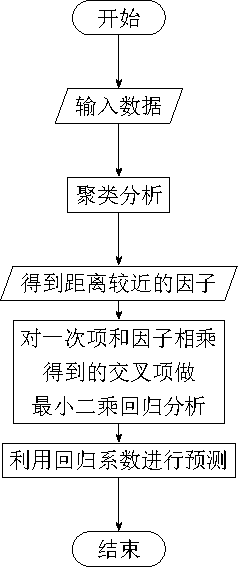
\includegraphics[height=0.6\linewidth]{dia.pdf}
	\caption{流程图}
	\label{fig:流程图}
\end{figure}

\subsection{假设}%
\label{sub:假设}

\begin{enumerate}
	\item 学生在填写附件中从南京回程购票信息调查表时均按照真实意愿和实际情况填写。
	\item 高铁及火车的价格、路线长度、行进速度、购票方式、舒适度在上次假期到下次寒假的时间段内不发生变化。
	\item 学生在考虑购买高铁还是火车时的思维方式、侧重点、偏好等在上次假期到下次寒假的时间段内不发生变化。
	\item 学生购票时不考虑自然灾害、人为破坏等情况对行进速度、舒适度等因素造成的影响。
\end{enumerate}

\section{问题一}%
\label{sec:问题一}
\subsection{筛选影响抉择结果的主要因素}
通过对文献进行研究,影响乘客选择高铁还是火车的因素主要来自两方面:一是客运方式选择的需求特性,与客运的主体(学生)有关;二是客运方式选择的供给特性,与交通运输方式有关。

综合以上两个层面的因素后,得到影响选择高铁还是火车的主要因素为:职业、出行目的、路程、收入水平、行进时间、票价、舒适度、安全性。

\subsection{\enquote{购票行为影响因素评价模型}}
我们使用R型聚类算法来评价乘客购票行为(结果)与这些因素之间关系。
\subsubsection{变量相似性度量}
我们使用相关系数来度量变量相似性。

记变量$x_j$的取值$(x_{1j},(x_{2j}, \cdots, (x_{nj})^\mathrm{T} \in  R^n(j=1,2,\cdots ,m)$。则可计算变量$x_j$和$x_k$的相关系数:
\begin{equation}
	r_{jk}=\frac{\sum\limits^n_{i=1} (x_{ij}- \overline{  x_{j}  })(x_{ik}-\overline{  x_{k}  })  }           { \sqrt{ \sum\limits^n_{i=1} {(x_{ij}-\overline{  x_{j}  })}^2     \sum\limits^n_{i=1} {(x_{ik}-\overline{  x_{k}  })}^2}}
\end{equation}

从而可以得到相关系数矩阵。

\subsubsection{变量聚类}
我们运用最长距离法对各因素聚类。定义两类变量的距离为:
\begin{equation}
	R(G_1,G_2)=\max\limits_{x_j \in G_1,x_k \in G_2}   \{d_{jk}\}
\end{equation}
式中:
\begin{equation}
	d_{jk}=1-|r_{jk}|
\end{equation}
或
\begin{equation}
	d^2_{jk}=1-r^2_{jk}
\end{equation}

\section{问题二}%
\label{sec:问题二}
\subsection{对\enquote{购票行为影响因素评价模型}的应用}

我们选区附件一中所列因素以及结果\enquote{选择高铁或火车}作为R型聚类因素,使用MATLAB软件编程得到聚类图:
\renewcommand\figurename{图}
\begin{figure}[H]
	\centering
	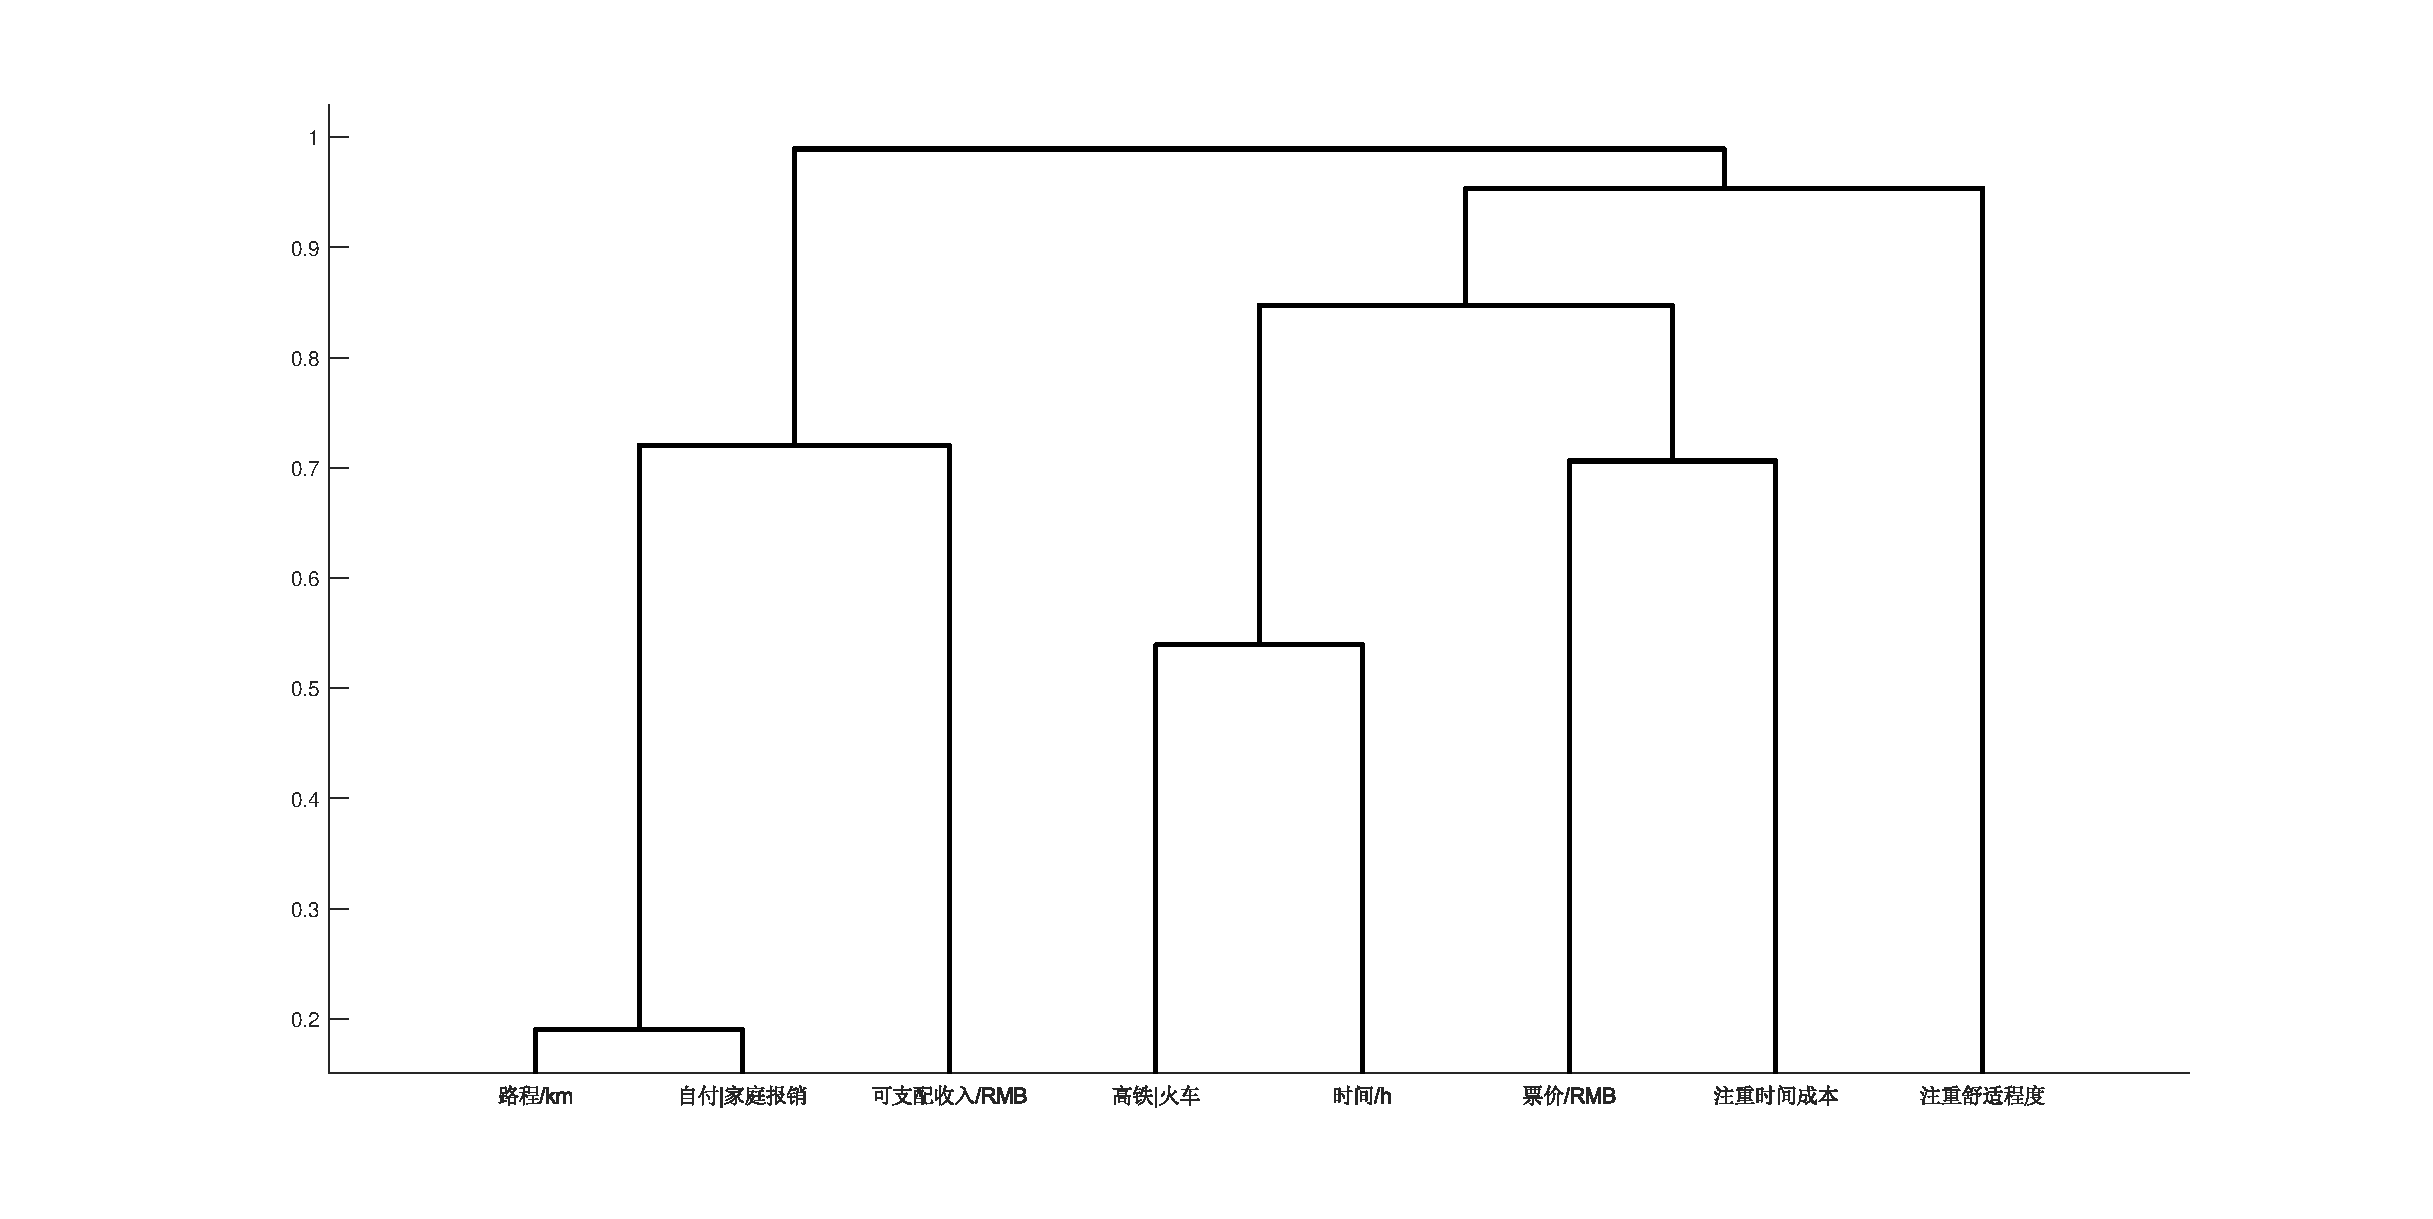
\includegraphics[width=.8\linewidth]{R.eps}
	\caption{聚类图} \label{all}
\end{figure}

从聚类图中可以看出,各个因素与\enquote{选择高铁还是火车}的相似性可以分为三档:
\begin{enumerate}
	\item 第一档(相似度最大):高铁/火车行程时间
	\item 第二档(相似度较大):票价
	\item 第三档(相似度较小):舒适程度
	\item 第四档(相似度较小):路程、自付/家庭报销、可支配收入
\end{enumerate}

可见,高铁/火车行程时间是影响抉择结果的最大因素。大部分大学生群体追求快节奏生活,不希望在路途中花费过多的时间,希望用最高效的方式来完成旅途。同时,行程时间短,也是高铁被发明的最初目的,也是它与火车相区别的主要因素。因此聚类结果符合大学生实际与生活实际。大学生对于时间的看重最大程度决定了对高铁还是火车的选择。由于高铁的时间更短,所以更加追求快速的学生会更倾向于高铁,而对速度不看重的同学会倾向于价格(第二档)低廉的火车。

\subsection{\enquote{购票行为预测模型}}
我们使用线性最小二乘回归算法,得到选择高铁还是火车与各个因素之间的定量关系。
\subsubsection{最小二乘法的基本原理}
已知一组数据,即平面上的$n$个点$(x_i,y_j),i=1,2, \cdots ,n$,$x_i$互不相同,寻求一个函数(曲线)$y=f(x)$,使得$f(x)$在某种准则下与所有数据点最为接近,则曲线拟合得最好。

而线性最小二乘法是解决曲线拟合最常用的方法,基本思路是,令:
\begin{equation}
	f(x)=a_1r_1(x)+a_2r_2(x)+ \cdots + a_mr_m(x)
\end{equation}
式中:

$r_k(x)$为事先选定好的一组线性无关的函数;

$a_k$为待定系数($k=1,2,\cdots ,m;m<n$)。

首先,应用上述\enquote{购票行为影响因素评价模型},得到对抉择影响最大的因素。随后,我们使用最小二乘回归算法,建立\enquote{购票行为预测模型}对影响抉择的因素从高到低排序,对影响抉择的因素及因素间关系进行量化分析。

\subsubsection{算法结果}
通过编程,我们确定了\enquote{乘坐高铁还是火车}作为因变量的拟合式中各个因素的系数:
\begin{table}[H]
	\centering
	\caption{拟合式中各个因素的系数以及截距}
	\renewcommand\arraystretch{1.4}

	\begin{tabular}{ccccp{13em}}
		\toprule
		标记&因素&单位&系数\\
		\midrule
		$x_1$&	注重时间成本&/&$0.19777$\\
		$x_2$&	可支配收入&RMB&	$0.060269$\\
		$x_3$&	票价&RMB&$	-0.05013$\\
		$x_4$&	票价$\times$注重时间成本&RMB&	$-0.047532$\\
		$x_5$&	时间&h&	$-0.041519$\\
		$x_6$&	自付/家庭报销&/&	$0.0017471$\\
		$x_7$&	注重舒适程度&/&	$4.26\times 10^{-5}$\\
		$x_8$&	路程&km&	$-8.64\times 10^{-6}$\\
		$x_9$&	路程$\times$自付/家庭报销&km&	$-2.83\times 10^{-7}$\\
		\bottomrule
	\end{tabular}
	\label{com}
\end{table}

截距:
\begin{equation}
	b=0.37519
\end{equation}

因此,若设决定\enquote{选择高铁还是火车}的指标为$Q$,则:
\begin{equation}
	Q=0.198x_1+0.060x_2-0.050x_3-0.048x_4-0.042x_5+0.00174x_6+4.26\times 10^{-5}x_7-8.64\times 10^{-6}x_8-2.83\times 1   \label{Q}
	0^{-7}x_9
\end{equation}

且从拟合结果可以看出,影响顾客购票行为的因素按从高到低排序为:

时间>可支配收入>票价>自付/家庭报销>舒适程度>路程

\subsubsection{判断选择高铁还是火车的准则}
若$Q \geqslant 0.5$,则预测选择乘坐高铁;

若$Q < 0.5$,则预测选择乘坐火车;

\section{问题三}%
\label{sec:问题三}
\subsection{计算\enquote{选择高铁还是火车}的指标$Q$}
利用附件2的数据,运用式\ref{Q},计算每位同学的$Q$值。

\subsection{得到每位同学出行方式的预测结果}
通过将$Q$与$0.5$进行比较,得到每位同学出行方式的预测结果。

在附件2的85名同学中,下一个寒假要购买高铁票的人数为68人,购买火车票的人数为17人。

购买高铁票的人数百分比为:
\begin{equation}
	\eta_1=\frac{68}{85}=80\%
\end{equation}

购买火车票的人数百分比为:
\begin{equation}
	\eta_1=\frac{17}{85}=20\%
\end{equation}

\section{问题四}%
\label{sec:问题四}
\subsection{计算每个省份乘坐高铁人数与乘坐火车人数之比}
为了能够得到对于前往不同地域,学生对高铁还是火车的选择的差别,我们分别计算了每个省份乘坐高铁人数与乘坐火车人数之比。
\begin{table}[H]
	\centering
	\caption{每个省份乘坐高铁人数与乘坐火车人数之比}
	\csvreader[
	head to column names,
	tabular=cc,
	table head=\toprule
	省份&高铁乘客人数/火车乘客人数比值
	\\
	\midrule,
	table foot=\bottomrule
	]{src/ratio.csv}{}{\csvcoli&\csvcolii}
\end{table}

从结果可以看出,从南京去往的省份距离南京越远,乘坐火车的比例越多;离南京越近,乘坐火车的人越多。

\begin{figure}[htpb]
	\centering
	\begin{subfigure}[htpb]{.45\linewidth}
		\centering
		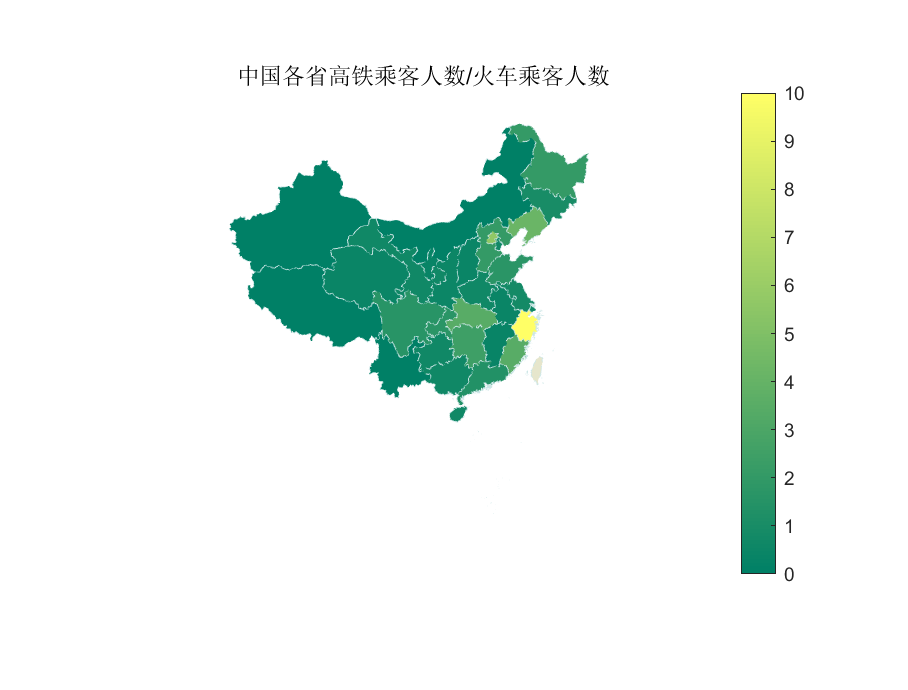
\includegraphics[width=0.8\linewidth]{map.eps}
		\caption{中国各省高铁、火车乘客人数之比地图}
		\label{fig:中国各省高铁、火车乘客人数之比地图}
	\end{subfigure}
	\quad
	\begin{subfigure}[htpb]{.45\linewidth}
		\centering
		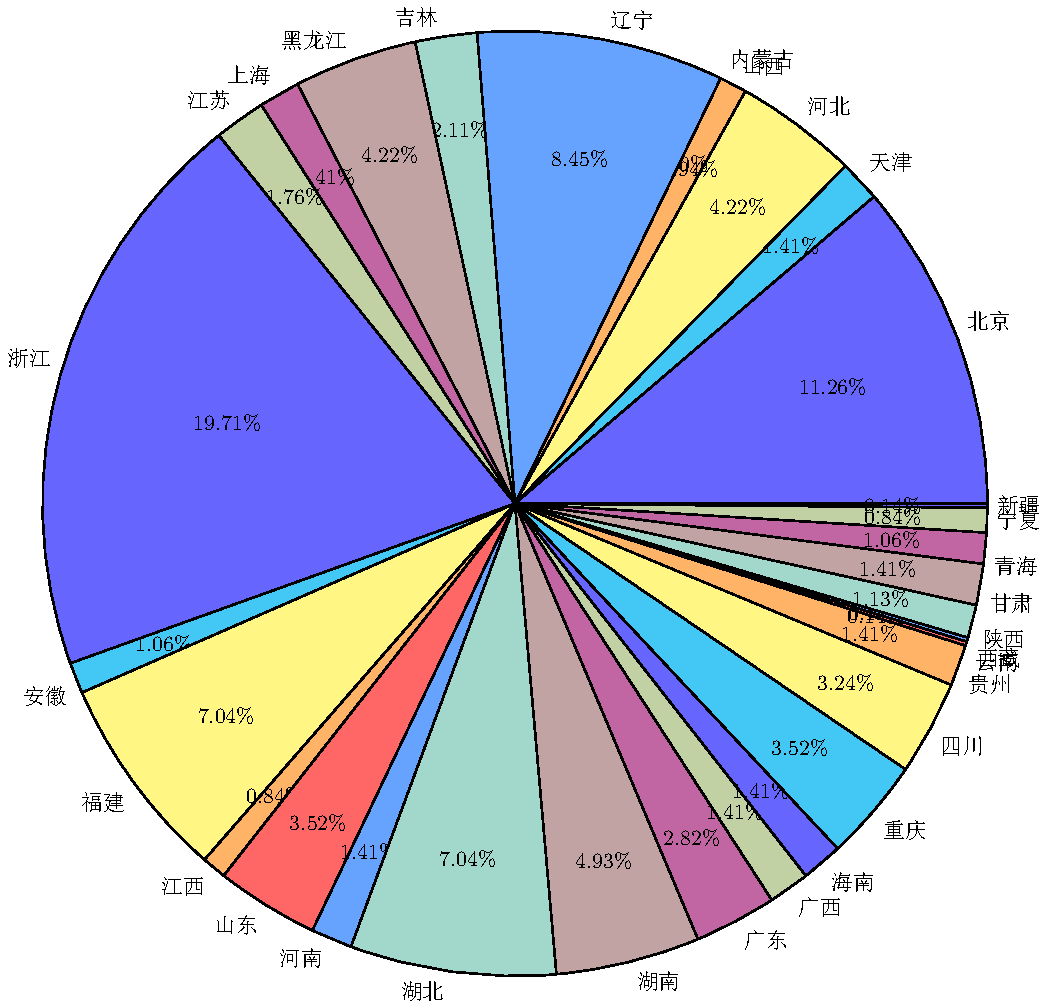
\includegraphics[width=0.8\linewidth]{pie.pdf}
		\caption{中国各省高铁、火车乘客人数之比饼状图}
		\label{fig:中国各省高铁、火车乘客人数之比饼状图}
	\end{subfigure}
	\quad
	\caption{中国各省高铁、火车乘客人数之比}
	\label{fig:中国各省高铁、火车乘客人数之比}
\end{figure}

\begin{tcolorbox}[colback=red!5!white,colframe=red!75!black,title=供铁路管理部门参考与决策的建议书,center title]
	\kaishu
	尊敬的铁路部门领导及工作人员:

	~~~~我们是三名本科学生组成的调研小组。近期,我们通过问卷调查及数学模型建立与运用,对我校学生从南京返程时选择乘坐高铁还是火车的行为决策进行了分析,研究了一定区域、特定阶段、并具有代表性人群的购票行为,分析高铁客运量与传统火车客运量的规律,得到了一些结论,并希望向铁路部门提出一些在高铁/火车数量安排等问题上的建议。

	~~~~首先,经过聚类分析,高铁/火车行程时间是影响大学生抉择乘坐高铁还是火车的最主要因素。大部分大学生群体追求快节奏生活,不希望在路途中花费过多的时间,希望用最高效的方式来完成旅途,因此会更加倾向于乘坐高铁。同时,行程时间短,也是高铁被发明的最初目的,也是它与火车相区别的主要因素。因此,我们建议铁路部门在保证安全的前提下通过改进高铁相关技术、优化运营线路等措施,提升高铁行进速度,从而满足更多学生返程的需求。

	~~~~第二,经过最小二乘法拟合,影响大学生购票行为的因素按从高到低排序为:时间$>$可支配收入$>$票价$>$自付/家庭报销$>$舒适程度$>$路程。可以发现,在排在首位的\enquote{时间}之后,连续三个因素都与金钱有关,表明大学生购买高铁还是火车很大程度上取决于票价、家庭经济状况及支付来源等。因此,我们建议铁路部门在上述\enquote{提升高铁行进速度的同时},减小技术成本,适当降低高铁票的价格,在为乘客提供快速旅行服务的同时,让更多大学生能够负担高铁的价格。

	~~~~最后,经过统计,从南京去往的省份距离南京越远,乘坐火车的比例越多;离南京越近,乘坐火车的人越多。这表明对于大学生而言,更倾向于短途高铁及长途火车。原因可能是随着距离的增加,高铁票价的增速大于火车票价的增速,长途高铁的价格非常昂贵,对于大学生来说出行成本太高。因此我们建议铁路部门可以适当降低长途高铁的票价,尤其寒假放假、暑假放假、国庆节放假等学生返乡高峰期,或增大学生票优惠力度,以满足更多学生需求。

	~~~~以上是我们对大学生选择乘坐高铁还是火车的行为决策进行的分析,以及有关建议,希望可以对铁路管理部门的管理工作提供参考与帮助,为学生返乡旅途提供更大的便利。如有不足,还望领导与工作人员扶正!

	~~~~谢谢您的阅读!

	\tcblower
	\kaishu
	\begin{flushright}
		学生调研小组

		\today
	\end{flushright}
\end{tcolorbox}

\section{模型的评价与改进}%
\label{sec:模型的评价与改进}

\subsection{优点}%
\label{sub:优点}
\begin{enumerate}
	\item 运用了R型聚类、最小二乘法等算法,通过客观数据得到结论。
	\item 最小二乘拟合使得\enquote{选择高铁还是火车}有了一个定量的判断准则,可以明确地预测学生下一寒假的出行方式。
\end{enumerate}

\subsection{缺点}%
\label{sub:缺点}
\begin{enumerate}
	\item 没有运用精确的算法来筛选影响购买高铁票还是火车票的主要因素,而是仅仅根据文献资料的结论。
	\item \enquote{选择高铁还是火车}的结果与各个因素之间的关系不一样符合线性关系,因此线性拟合得到的预测结果可能不准确。
	\item 在判断目标省份离南京的距离与选择高铁还是火车之间的关系时,有些省份没有开通高铁,或者有的省份的数据非常少,因此结果存在极端化情况,不够准确。
\end{enumerate}

\newpage

% Fakesection 参考文献

\bibliographystyle{IEEEtran}
\bibliography{src/main}

% Fakesection 附录

\renewcommand{\thesection}{\Alph{section}~}

\appendix

\section{代码}%
\label{sec:代码}

\langCVfile[Matlab][code:R.m][Matlab]{R.m}{src/R.m}

\begin{figure}[htpb]
	\centering
	\matlablightfile{MATLAB Command Window}{src/R.txt}
	\caption{运行界面}
	\label{fig:运行界面R.m}
\end{figure}

\langCVfile[Matlab][code:lsq.m][Matlab]{lsq.m}{src/lsq.m}

\begin{figure}[htpb]
	\centering
	\matlablightfile{MATLAB Command Window}{src/lsq.txt}
	\caption{运行界面}
	\label{fig:运行界面lsq.m}
\end{figure}

\langCVfile[Matlab][code:map.m][Matlab]{map.m}{src/map.m}

\begin{figure}[htpb]
	\centering
	\matlablightfile{MATLAB Command Window}{src/map.txt}
	\caption{运行界面}
	\label{fig:运行界面map.m}
\end{figure}

% Fakesection 索引

\printindex

\end{document}

